
\documentclass[border=5pt]{standalone}
\usepackage{xcolor}
\usepackage{tikz}
\usepackage{mathptmx}
\usetikzlibrary{
    positioning,
    calc
}
\tikzset{
    subfig/.style={
        line width = 2.5pt,
        align=center,
        % font=\LARGE
        font=\Huge
    },
}
\def\layerSpace{90mm}

\definecolor{VegetaRed}{HTML}{FFB6C1}
\definecolor{VegetaGreen}{HTML}{7FFFAA}

\begin{document}
    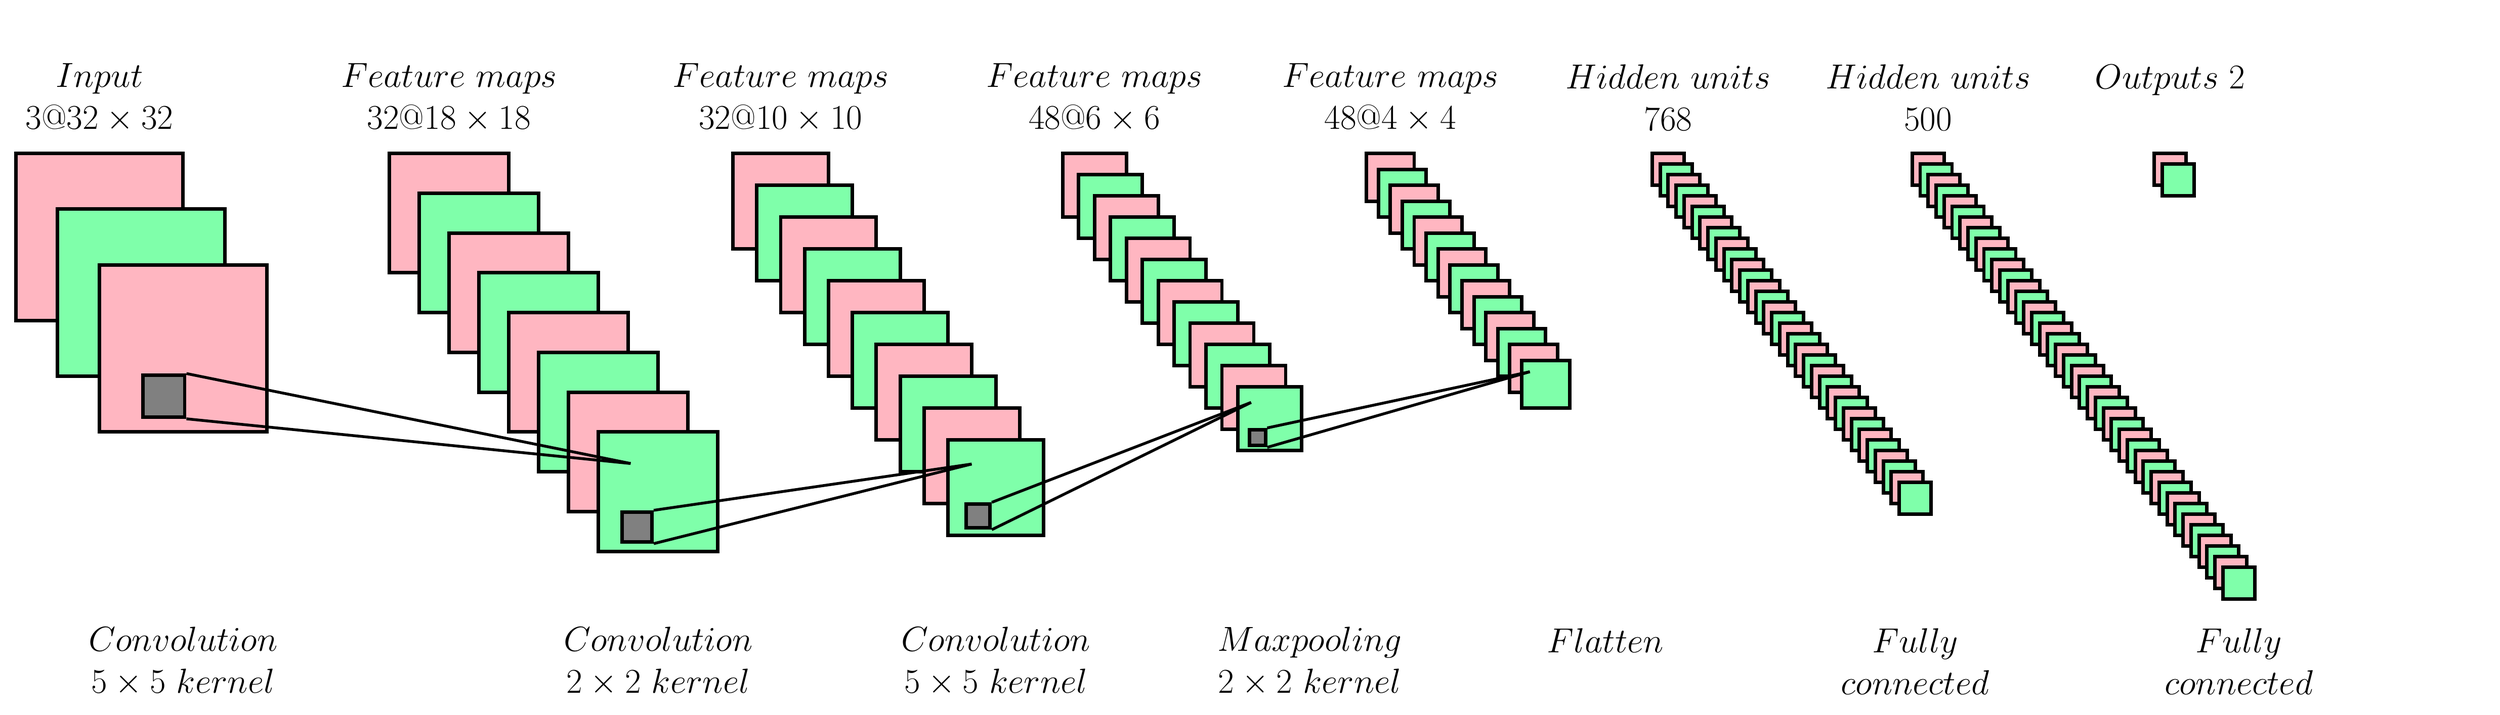
\begin{tikzpicture}
      % \newlength{\mytextlength}

                   \begin{scope}[xshift=0*\layerSpace]
                      % \settowidth{\mytextlength}{$Input\\ 3 @ 32\times 32$}
                       \coordinate (start) at (0,0);
                       \node [subfig,minimum width=42mm, minimum height=42mm] at ($(0,{42mm/2+4em})+(start)$) {$Input$\\ $ 3 @ 32\times 32$};
                       \foreach \i in {1,2,...,3}
                      {
                          \ifodd\i
                              \node [draw,fill=VegetaRed,subfig,minimum width=42mm, minimum height=42mm] at ($({42mm/4*(\i-1)},{-42mm/3*(\i-1)})+ (start)$) {};
                          \else
                              \node [draw,fill=VegetaGreen,subfig,minimum width=42mm, minimum height=42mm] at ($({42mm/4*(\i-1)},{-42mm/3*(\i-1)})+(start)$) {};
                          \fi
                      }
                      % \node (outmap0)[draw,fill=gray,subfig,minimum width=42mm*0.25, minimum height=42mm*0.25] at ($({(42mm/ 4*(3-1)) / 8 * 7},{(-42mm / 3*(3-1)) / 13 * 14})+(start)$) {};
                      \node (outmap0)[draw,fill=gray,subfig,minimum width=42mm*0.25, minimum height=42mm*0.25] at ($({(42mm/ 4*(3-1)) / (1+0.3)},{(-42mm / 3*(3-1)) / (1-0.3)})+(start)$) {};
                    \end{scope}
            
                       \begin{scope}[xshift=1*\layerSpace*(1-1/40)]
                          % \settowidth{\mytextlength}{$Feature~maps\\ 32 @ 18\times 18$}
                           \coordinate (start) at (0,6.0mm);
                           \node [subfig,minimum width=30mm, minimum height=30mm] at ($(0,{30mm/2+4em})+(start)$) {$Feature~maps$\\ $ 32 @ 18\times 18$};
                           \foreach \i in {1,2,...,8}
                          {
                              \ifodd\i
                                  \node [draw,fill=VegetaRed,subfig,minimum width=30mm, minimum height=30mm] at ($({30mm/4*(\i-1)},{-30mm/3*(\i-1)})+ (start)$) {};
                              \else
                                  \node [draw,fill=VegetaGreen,subfig,minimum width=30mm, minimum height=30mm] at ($({30mm/4*(\i-1)},{-30mm/3*(\i-1)})+(start)$) {};
                              \fi
                          }
                          \node (outmap1)[draw,fill=gray,subfig,minimum width=30mm*0.25, minimum height=30mm*0.25] at ($({(30mm/ 4*(8-1)) / (1+0.1125)},{(-30mm / 3*(8-1)) / (1-0.1125)})+(start)$) {};
                          % \node (inmap1)[draw,fill=gray,subfig,minimum width=30mm*0.15, minimum height=30mm*0.15] at ($({(30mm/ 4*(8-1)) / (1+0.1125)},{(-30mm / 3*(8-1)) / (1+0.1125)})+(start)$) {};
                          \node (inmap1)[subfig] at ($({(30mm/ 4*(8-1)) / (1+0.1125)},{(-30mm / 3*(8-1)) / (1+0.1125)})+(start)$) {};
                        \end{scope}
                
            \draw [line width=2pt](outmap0.south east) -- (inmap1.west);
            \draw [line width=2pt](outmap0.north east) -- (inmap1.west);
    
                       \begin{scope}[xshift=2*\layerSpace*(1-2/40)]
                          % \settowidth{\mytextlength}{$Feature~maps\\ 32 @ 10\times 10$}
                           \coordinate (start) at (0,9.0mm);
                           \node [subfig,minimum width=24mm, minimum height=24mm] at ($(0,{24mm/2+4em})+(start)$) {$Feature~maps$\\ $ 32 @ 10\times 10$};
                           \foreach \i in {1,2,...,10}
                          {
                              \ifodd\i
                                  \node [draw,fill=VegetaRed,subfig,minimum width=24mm, minimum height=24mm] at ($({24mm/4*(\i-1)},{-24mm/3*(\i-1)})+ (start)$) {};
                              \else
                                  \node [draw,fill=VegetaGreen,subfig,minimum width=24mm, minimum height=24mm] at ($({24mm/4*(\i-1)},{-24mm/3*(\i-1)})+(start)$) {};
                              \fi
                          }
                          \node (outmap2)[draw,fill=gray,subfig,minimum width=24mm*0.25, minimum height=24mm*0.25] at ($({(24mm/ 4*(10-1)) / (1+0.09)},{(-24mm / 3*(10-1)) / (1-0.09)})+(start)$) {};
                          % \node (inmap2)[draw,fill=gray,subfig,minimum width=24mm*0.15, minimum height=24mm*0.15] at ($({(24mm/ 4*(10-1)) / (1+0.09)},{(-24mm / 3*(10-1)) / (1+0.09)})+(start)$) {};
                          \node (inmap2)[subfig] at ($({(24mm/ 4*(10-1)) / (1+0.09)},{(-24mm / 3*(10-1)) / (1+0.09)})+(start)$) {};
                        \end{scope}
                
            \draw [line width=2pt](outmap1.south east) -- (inmap2.west);
            \draw [line width=2pt](outmap1.north east) -- (inmap2.west);
    
                       \begin{scope}[xshift=3*\layerSpace*(1-3/40)]
                          % \settowidth{\mytextlength}{$Feature~maps\\ 48 @ 6\times 6$}
                           \coordinate (start) at (0,13.0mm);
                           \node [subfig,minimum width=16mm, minimum height=16mm] at ($(0,{16mm/2+4em})+(start)$) {$Feature~maps$\\ $ 48 @ 6\times 6$};
                           \foreach \i in {1,2,...,12.0}
                          {
                              \ifodd\i
                                  \node [draw,fill=VegetaRed,subfig,minimum width=16mm, minimum height=16mm] at ($({16mm/4*(\i-1)},{-16mm/3*(\i-1)})+ (start)$) {};
                              \else
                                  \node [draw,fill=VegetaGreen,subfig,minimum width=16mm, minimum height=16mm] at ($({16mm/4*(\i-1)},{-16mm/3*(\i-1)})+(start)$) {};
                              \fi
                          }
                          \node (outmap3)[draw,fill=gray,subfig,minimum width=16mm*0.25, minimum height=16mm*0.25] at ($({(16mm/ 4*(12.0-1)) / (1+0.075)},{(-16mm / 3*(12.0-1)) / (1-0.075)})+(start)$) {};
                          % \node (inmap3)[draw,fill=gray,subfig,minimum width=16mm*0.15, minimum height=16mm*0.15] at ($({(16mm/ 4*(12.0-1)) / (1+0.075)},{(-16mm / 3*(12.0-1)) / (1+0.075)})+(start)$) {};
                          \node (inmap3)[subfig] at ($({(16mm/ 4*(12.0-1)) / (1+0.075)},{(-16mm / 3*(12.0-1)) / (1+0.075)})+(start)$) {};
                        \end{scope}
                
            \draw [line width=2pt](outmap2.south east) -- (inmap3.west);
            \draw [line width=2pt](outmap2.north east) -- (inmap3.west);
    
                       \begin{scope}[xshift=4*\layerSpace*(1-4/40)]
                          % \settowidth{\mytextlength}{$Feature~maps\\ 48 @ 4\times 4$}
                           \coordinate (start) at (0,15.0mm);
                           \node [subfig,minimum width=12mm, minimum height=12mm] at ($(0,{12mm/2+4em})+(start)$) {$Feature~maps$\\ $ 48 @ 4\times 4$};
                           \foreach \i in {1,2,...,14.0}
                          {
                              \ifodd\i
                                  \node [draw,fill=VegetaRed,subfig,minimum width=12mm, minimum height=12mm] at ($({12mm/4*(\i-1)},{-12mm/3*(\i-1)})+ (start)$) {};
                              \else
                                  \node [draw,fill=VegetaGreen,subfig,minimum width=12mm, minimum height=12mm] at ($({12mm/4*(\i-1)},{-12mm/3*(\i-1)})+(start)$) {};
                              \fi
                          }
                          % \node (outmap4)[draw,fill=gray,subfig,minimum width=12mm*0.25, minimum height=12mm*0.25] at ($({(12mm/ 4*(14.0-1)) / (1+0.0642857142857143)},{(-12mm / 3*(14.0-1)) / (1-0.0642857142857143)})+(start)$) {};
                          % \node (inmap4)[draw,fill=gray,subfig,minimum width=12mm*0.15, minimum height=12mm*0.15] at ($({(12mm/ 4*(14.0-1)) / (1+0.0642857142857143)},{(-12mm / 3*(14.0-1)) / (1+0.0642857142857143)})+(start)$) {};
                          \node (inmap4)[subfig] at ($({(12mm/ 4*(14.0-1)) / (1+0.0642857142857143)},{(-12mm / 3*(14.0-1)) / (1+0.0642857142857143)})+(start)$) {};
                        \end{scope}
                
            \draw [line width=2pt](outmap3.south east) -- (inmap4.west);
            \draw [line width=2pt](outmap3.north east) -- (inmap4.west);
    
           \begin{scope}[xshift=5*\layerSpace*(1-5/40)]
               \coordinate (start) at (0,17.0mm);
               \node [subfig,minimum width=8mm, minimum height=8mm] at ($(0,{8mm/2+4em})+(start)$) {$Hidden~units$\\ $ 768$};
               \foreach \i in {1,2,...,32}
              {
                  \ifodd\i
                      \node [draw,fill=VegetaRed,subfig,minimum width=8mm, minimum height=8mm] at ($({8mm/4*(\i-1)},{-8mm/3*(\i-1)})+ (start)$) {};
                  \else
                      \node [draw,fill=VegetaGreen,subfig,minimum width=8mm, minimum height=8mm] at ($({8mm/4*(\i-1)},{-8mm/3*(\i-1)})+(start)$) {};
                  \fi
              }
            \end{scope}
    
           \begin{scope}[xshift=6*\layerSpace*(1-6/40)]
               \coordinate (start) at (0,17.0mm);
               \node [subfig,minimum width=8mm, minimum height=8mm] at ($(0,{8mm/2+4em})+(start)$) {$Hidden~units$\\ $ 500$};
               \foreach \i in {1,2,...,40}
              {
                  \ifodd\i
                      \node [draw,fill=VegetaRed,subfig,minimum width=8mm, minimum height=8mm] at ($({8mm/4*(\i-1)},{-8mm/3*(\i-1)})+ (start)$) {};
                  \else
                      \node [draw,fill=VegetaGreen,subfig,minimum width=8mm, minimum height=8mm] at ($({8mm/4*(\i-1)},{-8mm/3*(\i-1)})+(start)$) {};
                  \fi
              }
            \end{scope}
    
           \begin{scope}[xshift=7*\layerSpace*(1-7/40)]
               \coordinate (start) at (0,17.0mm);
               \node [subfig,minimum width=8mm, minimum height=8mm] at ($(0,{8mm/2+4em})+(start)$) {$Outputs~2$\\ $ $};
               \foreach \i in {1,2,...,2}
              {
                  \ifodd\i
                      \node [draw,fill=VegetaRed,subfig,minimum width=8mm, minimum height=8mm] at ($({8mm/4*(\i-1)},{-8mm/3*(\i-1)})+ (start)$) {};
                  \else
                      \node [draw,fill=VegetaGreen,subfig,minimum width=8mm, minimum height=8mm] at ($({8mm/4*(\i-1)},{-8mm/3*(\i-1)})+(start)$) {};
                  \fi
              }
            \end{scope}
    
           \node [subfig] at ($({21.0mm+0*\layerSpace*(1-0/40)},{-106.66666666666666mm})$) {$Convolution$\\ $ 5\times 5~kernel$};

           \node [subfig] at ($({52.5mm+1*\layerSpace*(1-1/40)},{-106.66666666666666mm})$) {$Convolution$\\ $ 2\times 2~kernel$};

           \node [subfig] at ($({54.0mm+2*\layerSpace*(1-2/40)},{-106.66666666666666mm})$) {$Convolution$\\ $ 5\times 5~kernel$};

           \node [subfig] at ($({54.0mm+3*\layerSpace*(1-3/40)},{-106.66666666666666mm})$) {$Maxpooling$\\ $ 2\times 2~kernel$};

           \node [subfig] at ($({54.0mm+4*\layerSpace*(1-4/40)},{-106.66666666666666mm})$) {$Flatten$\\ $ $};

           \node [subfig] at ($({62.0mm+5*\layerSpace*(1-5/40)},{-106.66666666666666mm})$) {$Fully$\\ $ connected$};

           \node [subfig] at ($({78.0mm+6*\layerSpace*(1-6/40)},{-106.66666666666666mm})$) {$Fully$\\ $ connected$};

           \node [subfig] at ($({78.0mm+7*\layerSpace*(1-7/40)},{-106.66666666666666mm})$) {$ $\\ $ $};

    \end{tikzpicture}
\end{document}
